\documentclass{beamer}
\usepackage{graphicx}

\title{Platform Autoscaling Dev Demo}
\subtitle{It's here.}
\author{Troy Sankey}
\date{\today}

\begin{document}

\begin{frame}
\titlepage
\end{frame}

\begin{frame}
\frametitle{Configuration}
\setbeamercovered{invisible}
\begin{itemize}
\item Initially, the instance count was 12, now we scale between 6 and 12.
% mention AZs.
\item Average CPUUtilization is controlled to stay between 35\% and 55\%.
\item 10 minute instance launch delay.
\end{itemize}
\end{frame}

\begin{frame}
\frametitle{Stability}
\begin{center}
Instance Count
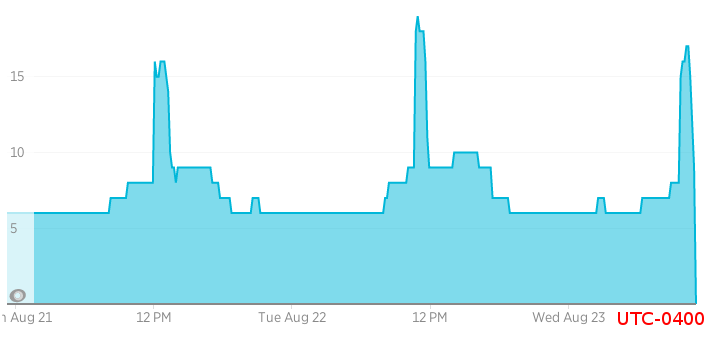
\includegraphics[width=\textwidth]{instance_count.png}
\end{center}
\end{frame}

\begin{frame}
\frametitle{Stability}
\begin{center}
Instance Count
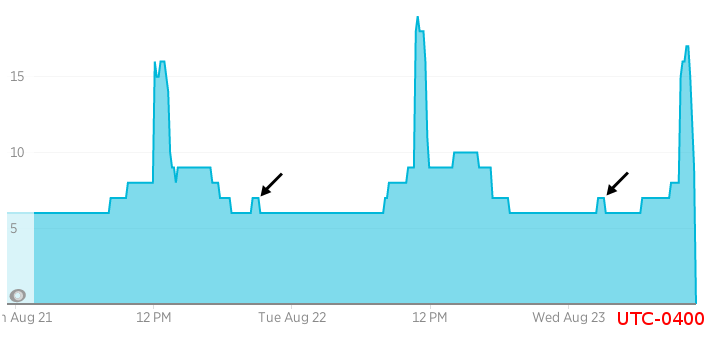
\includegraphics[width=\textwidth]{instance_count_arrows.png}
\end{center}
\end{frame}

\begin{frame}
\frametitle{Stability}
\begin{center}
Throughput (requests/minute)
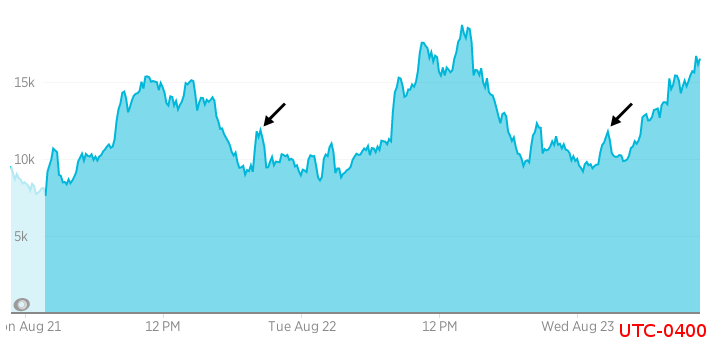
\includegraphics[width=\textwidth]{throughput_arrows.png}
\end{center}
\end{frame}

\begin{frame}
\frametitle{Cost}
\setbeamercovered{invisible}
\begin{itemize}
\item Average of 6.8 instance over the last week
\item Initial yearly cost savings of about \$10,000, after adjusting reservations from 12 to 6 instances.
% After adjusting reservations, and for one cluster.
% ((0.252 (1/hour) * 12) - (0.252 (1/hour) * 6) - (0.398 (1/hour) * 0.78)) * 1 year
\end{itemize}
\end{frame}

\begin{frame}
\frametitle{Woes}
\setbeamercovered{invisible}
\begin{itemize}
\item About 4ms increase in median response time (+10\%).
\end{itemize}
\end{frame}

\end{document}
